%iffalse
\let\negmedspace\undefined
\let\negthickspace\undefined
\documentclass[journal,12pt,onecolumn]{IEEEtran}
\usepackage{cite}
\usepackage{amsmath,amssymb,amsfonts,amsthm}
\usepackage{algorithmic}
\usepackage{graphicx}
\usepackage{textcomp}
\usepackage{xcolor}
\usepackage{txfonts}
\usepackage{listings}
\usepackage{enumitem}
\usepackage{mathtools}
\usepackage{gensymb}
\usepackage{comment}
\usepackage[breaklinks=true]{hyperref}
\usepackage{tkz-euclide} 
\usepackage{listings}

\usepackage{booktabs}
\usepackage{pgfplots}
\usepackage{gvv}                                        
\usepackage[latin1]{inputenc}     
\usepackage{xparse}
\usepackage{color}                                            
\usepackage{array}                                            
\usepackage{longtable}                                       
\usepackage{calc}                                             
\usepackage{multirow}
\usepackage{multicol}
\usepackage{hhline}                                           
\usepackage{ifthen}                                           
\usepackage{lscape}
\usepackage{tabularx}
\usepackage{array}
\usetikzlibrary{patterns}
\usepackage{siunitx}
\pagestyle{empty}
\usetikzlibrary{calc}
\usepackage[margin=1in]{geometry}
\usepackage{pgffor}
\usepackage{float}
\usepackage{pgf-pie}
\newtheorem{theorem}{Theorem}[section]
\newtheorem{problem}{Problem}
\newtheorem{proposition}{Proposition}[section]
\newtheorem{lemma}{Lemma}[section]
\newtheorem{corollary}[theorem]{Corollary}
\newtheorem{example}{Example}[section]
\newtheorem{definition}[problem]{Definition}
\newcommand{\BEQA}{\begin{eqnarray}}
\newcommand{\EEQA}{\end{eqnarray}}
\newcommand{\define}{\stackrel{\triangle}{=}}
\theoremstyle{remark}
\newtheorem{rem}{Remark}
% Marks the beginning of the document
\pgfplotsset{compat=1.18}
\begin{document}



\bibliographystyle{IEEEtran}
\vspace{3cm}


\title{2023-ST-'1-13'}
\author{EE24BTECH11023}
%\maketitle
%\newpage
%\bigskip
\maketitle




{\let\newpage\relax\maketitle}

\renewcommand{\thefigure}{\theenumi}
\renewcommand{\thetable}{\theenumi}
\setlength{\intextsep}{10pt} % Space between text and floats


\numberwithin{equation}{enumi}
\numberwithin{figure}{enumi}
\renewcommand{\thetable}{\theenumi}


\begin{enumerate}

    \item "I have not yet decided what I will do this evening; I {\underline{\hspace{2cm}}}visit a friend."
    \begin{enumerate}
        \item mite
        \item would
        \item might
        \item didn't
    \end{enumerate}

    \item Eject : Insert :: Advance :\\
    (By word meaning)
    
    \begin{enumerate}
        \item Advent
        \item Progress
        \item Retreat
        \item Loan
    \end{enumerate}

    \item In the given figure, $PQRSTV$ is a regular hexagon with each side of length $5$ cm. A circle is drawn with its center at $V$ such that it passes through $P$. What is the area (in $cm^2$) of the shaded region?(The diagram is representative)

    \begin{enumerate}
        \item $\frac{25\pi}{3}$
        \item $\frac{20\pi}{3}$
        \item $6\pi$
        \item $7\pi$
    \end{enumerate}

    \begin{figure}[H]
        \centering
        
    \centering
    \begin{tabular}{|c|c|c|}
        \hline
        \textbf{Activity} & \textbf{Time (hours)} & \textbf{Immediate predecessors} \\
        \hline
        A & 2 & -- \\
        \hline
        B & 3 & -- \\
                \hline
        C & 2 & -- \\
        \hline
        D & 4 & A \\
        \hline
        E & 5 & B \\
        \hline
        F & 4 & B \\
        \hline
        G & 3 & C \\
        \hline
        H & 10 & D, E \\
        \hline
        I & 5 & F \\
        \hline
        J & 8 & G \\
        \hline
        K & 3 & H, I, J \\
        \hline
    \end{tabular}

  % Use the correct path to your Q4.tex file
    \end{figure}


    \item A duck named Donald Duck says "All ducks always lie." \\
    Based only on the information above, which one of the following statements can be logically inferred with certainty?
    \begin{enumerate}
        \item Donald Duck always lies.
        \item Donald Duck always tells the truth.
        \item Donald Duck's statement is true.
        \item Donald Duck's statement is false.
    \end{enumerate}

    \item A line of symmetry is defined as a line that divides a figure into two parts in a way such that each part is a mirror image of the other part about that line.\\
    The figure below consists of $20$ unit squares arranged as shown. In addition to the given black squares, up to $5$ more may be colored black. Which one among the following options depicts the minimum number of boxes that must be colored black to achieve two lines of symmetry?(The figure is representative)
\begin{figure}[H]
        \centering
        
    \begin{tabular}{cc}
        \toprule
        \( f \) (MPa) & Number of specimens with \\
                      & compressive strength equal to \( f \) \\
        \midrule
        23   & 4 \\
        28   & 2 \\
        22.5 & 5 \\
        31   & 5 \\
        29   & 4 \\
        \bottomrule
    \end{tabular}
  % Use the correct path to your Q4.tex file
    \end{figure}
    
    \begin{enumerate}
        \item d
        \item c, d, i
        \item c,i
        \item c, d, i, f, g
    \end{enumerate}

    \item Based only on the truth of the statement "Some humans are intelligent," which one of the following options can be logically inferred with certainty?
    \begin{enumerate}
        \item No human is intelligent.
        \item All humans are intelligent.
        \item Some non-humans are intelligent.
        \item Some intelligent beings are humans.
    \end{enumerate}

    \item Which one of the options can be inferred about the mean, median, and mode for the given probability distribution ($i.e.$ probability mass function ),$P(x)$, of a variable $x$?
      \begin{figure}[H]
        \centering
        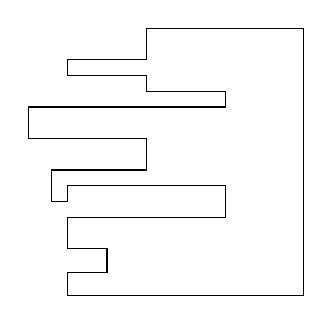
\begin{tikzpicture}
        \draw (0,0.6) -- (3,0.6) -- (3,4) -- (1,4) -- (1,3.6) -- (0,3.6) -- (0,3.4) -- (1,3.4) --  (1,3.2) -- (2,3.2) -- (2,3) -- (-0.5,3)--(-0.5,2.6) -- (1,2.6) -- (1,2.2) -- (-0.2,2.2) -- (-0.2,1.8) -- (0,1.8) -- (0,2) --  (2,2) -- (2,1.6) -- (0,1.6) -- (0,1.2)--(0.5,1.2)--(0.5,0.9)--(0,0.9) -- cycle;
    \end{tikzpicture}

  % Use the correct path to your Q4.tex file
    \end{figure}
    \begin{enumerate}
        \item mean = median $\neq$ mode
        \item mean = median = mode
        \item mean $\neq$ median = mode
        \item mean $\neq$ mode = median
    \end{enumerate}

    \item The James Webb telescope, recently launched in space, is giving humankind unprecedented access to the depths of time by imaging very old stars formed almost $13$ billion years ago. Astrophysicists and cosmologists believe that this odyssey in space may even shed light on the existence of dark matter. Dark matter is supposed to interact only via the gravitational interaction and not through electromagnetic, weak, or strong interactions. This may justify the epithet "dark" in dark matter.

     Based on the following paragraph, which one of the statements is FALSE? 

    \begin{enumerate}
        \item No other telescope has captured images of stars older than those captured by the James Webb telescope.
        \item People other than astrophysicists and cosmologists may also believe in the existence of dark matter.
        \item The James Webb telescope could be of use in the research on dark matter.
        \item If dark matter was known to interact via the strong interaction, then the epithet "dark" would be justified.
    \end{enumerate}

    \item Let $a = 30!$, $b = 50!$, and $c = 100!$. Consider the following numbers:\\ 
    $\log_a a$, $\log_b a$, $\log_c a$,$\log_a b$\\
    Which one of the following inequalities is CORRECT?
    \begin{enumerate}
        \item $\log_c a < \log_b a < \log_a b < \log_a c$
        \item $\log_c a < \log_a b < \log_b a < \log_b c$
        \item $\log_c a < \log_b a < \log_a c < \log_a b$
        \item $\log_b a < \log_c a < \log_a b < \log_a c$
    \end{enumerate}

    \item A square of side length $4$ cm is given. The boundary of the shaded region is defined by one semi-circle on the top and two circular arcs at the bottom, each of radius $2$ cm, as shown.
      \begin{figure}[H]
        \centering
        
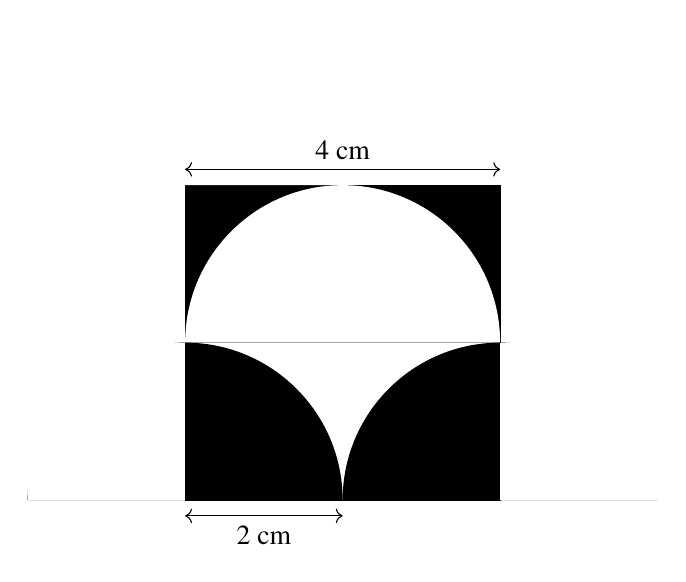
\begin{tikzpicture}
    % Draw the square
    \draw[fill=white] (0,0) rectangle (4,4);
    \fill[fill=black] (0,2) rectangle (4,4);
    \fill[white] (4,2) arc[start angle=0, end angle=180, radius=2cm] -- cycle;
   

    \fill[white] (2,4) arc[start angle=0, end angle=180, radius=2cm] -- cycle;

    % Bottom left and right semicircles
    \fill[black] (2,0) arc[start angle=0, end angle=180, radius=2cm] -- cycle;
    \fill[black] (6,0) arc[start angle=0, end angle=180, radius=2cm] -- cycle;
 \fill[fill=white] (-2,0) rectangle (0,2);
    \fill[fill=white] (4,0) rectangle (6,2);
    % Labels for dimensions
    \draw[<->] (0,4.2) -- (4,4.2) node[midway, above] {4 cm};
    \draw[<->] (0,-0.2) -- (2,-0.2) node[midway, below] {2 cm};
\end{tikzpicture}

  % Use the correct path to your Q4.tex file
    \end{figure}
    The area of the shaded region is {\underline{\hspace{2cm}}}$cm^2$.
    \begin{enumerate}
        \item $8$
        \item $4$
        \item $12$ 
        \item $2$
    \end{enumerate}


    \item The area of the region bounded by the parabola $x = -y^2$ and the line $y = x + 2$ equals
    \begin{enumerate}
        \item $\frac{3}{2}$
        \item $\frac{7}{2}$
        \item $\frac{9}{2}$
        \item $9$
    \end{enumerate}

    \item Let $A$ be a $3 \times 3$ real matrix having eigenvalues $1$, $0$, and $-1$. If $B = A^2 + 2A + I_3$, where $I_3$ is the $3 \times 3$ identity matrix, then which one of the following statements is true?
    \begin{enumerate}
        \item $B^3 - 5B^2 + 4B = 0$
        \item $B^3 - 5B^2 - 4B = 0$
        \item $B^3 + 5B^2 - 4B = 0$
        \item $B^3 + 5B^2 + 4B = 0$
    \end{enumerate}

    \item Consider the following statements.
    \begin{enumerate}
    \item[(I)] Let $A$ and $B$ be two $n \times n$ real matrices. If $B$ is invertible, then $\text{rank}(BA) = \text{rank}(A)$.
    \item[(II)] Let $A$ be an $n \times n$ real matrix.If $A^2x=b$ has a solution for every $b\in R^n$ ,then $Ax=b$ also has a solution for every $b\in R^n$.
    \end{enumerate}

    Which of the following is/are true?
    \begin{enumerate}
        \item Only (I)
        \item Only (II)
        \item Both (I) and (II)
        \item Neither (I) nor (II)
    \end{enumerate}

\end{enumerate}
\end{document}